% Options for packages loaded elsewhere
\PassOptionsToPackage{unicode}{hyperref}
\PassOptionsToPackage{hyphens}{url}
%
\documentclass[
]{article}
\usepackage{amsmath,amssymb}
\usepackage{lmodern}
\usepackage{iftex}
\ifPDFTeX
  \usepackage[T1]{fontenc}
  \usepackage[utf8]{inputenc}
  \usepackage{textcomp} % provide euro and other symbols
\else % if luatex or xetex
  \usepackage{unicode-math}
  \defaultfontfeatures{Scale=MatchLowercase}
  \defaultfontfeatures[\rmfamily]{Ligatures=TeX,Scale=1}
\fi
% Use upquote if available, for straight quotes in verbatim environments
\IfFileExists{upquote.sty}{\usepackage{upquote}}{}
\IfFileExists{microtype.sty}{% use microtype if available
  \usepackage[]{microtype}
  \UseMicrotypeSet[protrusion]{basicmath} % disable protrusion for tt fonts
}{}
\makeatletter
\@ifundefined{KOMAClassName}{% if non-KOMA class
  \IfFileExists{parskip.sty}{%
    \usepackage{parskip}
  }{% else
    \setlength{\parindent}{0pt}
    \setlength{\parskip}{6pt plus 2pt minus 1pt}}
}{% if KOMA class
  \KOMAoptions{parskip=half}}
\makeatother
\usepackage{xcolor}
\usepackage[margin=1in]{geometry}
\usepackage{color}
\usepackage{fancyvrb}
\newcommand{\VerbBar}{|}
\newcommand{\VERB}{\Verb[commandchars=\\\{\}]}
\DefineVerbatimEnvironment{Highlighting}{Verbatim}{commandchars=\\\{\}}
% Add ',fontsize=\small' for more characters per line
\usepackage{framed}
\definecolor{shadecolor}{RGB}{248,248,248}
\newenvironment{Shaded}{\begin{snugshade}}{\end{snugshade}}
\newcommand{\AlertTok}[1]{\textcolor[rgb]{0.94,0.16,0.16}{#1}}
\newcommand{\AnnotationTok}[1]{\textcolor[rgb]{0.56,0.35,0.01}{\textbf{\textit{#1}}}}
\newcommand{\AttributeTok}[1]{\textcolor[rgb]{0.77,0.63,0.00}{#1}}
\newcommand{\BaseNTok}[1]{\textcolor[rgb]{0.00,0.00,0.81}{#1}}
\newcommand{\BuiltInTok}[1]{#1}
\newcommand{\CharTok}[1]{\textcolor[rgb]{0.31,0.60,0.02}{#1}}
\newcommand{\CommentTok}[1]{\textcolor[rgb]{0.56,0.35,0.01}{\textit{#1}}}
\newcommand{\CommentVarTok}[1]{\textcolor[rgb]{0.56,0.35,0.01}{\textbf{\textit{#1}}}}
\newcommand{\ConstantTok}[1]{\textcolor[rgb]{0.00,0.00,0.00}{#1}}
\newcommand{\ControlFlowTok}[1]{\textcolor[rgb]{0.13,0.29,0.53}{\textbf{#1}}}
\newcommand{\DataTypeTok}[1]{\textcolor[rgb]{0.13,0.29,0.53}{#1}}
\newcommand{\DecValTok}[1]{\textcolor[rgb]{0.00,0.00,0.81}{#1}}
\newcommand{\DocumentationTok}[1]{\textcolor[rgb]{0.56,0.35,0.01}{\textbf{\textit{#1}}}}
\newcommand{\ErrorTok}[1]{\textcolor[rgb]{0.64,0.00,0.00}{\textbf{#1}}}
\newcommand{\ExtensionTok}[1]{#1}
\newcommand{\FloatTok}[1]{\textcolor[rgb]{0.00,0.00,0.81}{#1}}
\newcommand{\FunctionTok}[1]{\textcolor[rgb]{0.00,0.00,0.00}{#1}}
\newcommand{\ImportTok}[1]{#1}
\newcommand{\InformationTok}[1]{\textcolor[rgb]{0.56,0.35,0.01}{\textbf{\textit{#1}}}}
\newcommand{\KeywordTok}[1]{\textcolor[rgb]{0.13,0.29,0.53}{\textbf{#1}}}
\newcommand{\NormalTok}[1]{#1}
\newcommand{\OperatorTok}[1]{\textcolor[rgb]{0.81,0.36,0.00}{\textbf{#1}}}
\newcommand{\OtherTok}[1]{\textcolor[rgb]{0.56,0.35,0.01}{#1}}
\newcommand{\PreprocessorTok}[1]{\textcolor[rgb]{0.56,0.35,0.01}{\textit{#1}}}
\newcommand{\RegionMarkerTok}[1]{#1}
\newcommand{\SpecialCharTok}[1]{\textcolor[rgb]{0.00,0.00,0.00}{#1}}
\newcommand{\SpecialStringTok}[1]{\textcolor[rgb]{0.31,0.60,0.02}{#1}}
\newcommand{\StringTok}[1]{\textcolor[rgb]{0.31,0.60,0.02}{#1}}
\newcommand{\VariableTok}[1]{\textcolor[rgb]{0.00,0.00,0.00}{#1}}
\newcommand{\VerbatimStringTok}[1]{\textcolor[rgb]{0.31,0.60,0.02}{#1}}
\newcommand{\WarningTok}[1]{\textcolor[rgb]{0.56,0.35,0.01}{\textbf{\textit{#1}}}}
\usepackage{graphicx}
\makeatletter
\def\maxwidth{\ifdim\Gin@nat@width>\linewidth\linewidth\else\Gin@nat@width\fi}
\def\maxheight{\ifdim\Gin@nat@height>\textheight\textheight\else\Gin@nat@height\fi}
\makeatother
% Scale images if necessary, so that they will not overflow the page
% margins by default, and it is still possible to overwrite the defaults
% using explicit options in \includegraphics[width, height, ...]{}
\setkeys{Gin}{width=\maxwidth,height=\maxheight,keepaspectratio}
% Set default figure placement to htbp
\makeatletter
\def\fps@figure{htbp}
\makeatother
\setlength{\emergencystretch}{3em} % prevent overfull lines
\providecommand{\tightlist}{%
  \setlength{\itemsep}{0pt}\setlength{\parskip}{0pt}}
\setcounter{secnumdepth}{-\maxdimen} % remove section numbering
\ifLuaTeX
  \usepackage{selnolig}  % disable illegal ligatures
\fi
\IfFileExists{bookmark.sty}{\usepackage{bookmark}}{\usepackage{hyperref}}
\IfFileExists{xurl.sty}{\usepackage{xurl}}{} % add URL line breaks if available
\urlstyle{same} % disable monospaced font for URLs
\hypersetup{
  pdftitle={Untitled},
  hidelinks,
  pdfcreator={LaTeX via pandoc}}

\title{Untitled}
\author{}
\date{\vspace{-2.5em}2022-09-14}

\begin{document}
\maketitle

\begin{Shaded}
\begin{Highlighting}[]
\FunctionTok{library}\NormalTok{(binom)}
\FunctionTok{library}\NormalTok{(car)}
\end{Highlighting}
\end{Shaded}

\begin{verbatim}
## Loading required package: carData
\end{verbatim}

\begin{Shaded}
\begin{Highlighting}[]
\FunctionTok{library}\NormalTok{(collapsibleTree)}
\FunctionTok{library}\NormalTok{(dbplyr)}
\FunctionTok{library}\NormalTok{(dplyr)}
\end{Highlighting}
\end{Shaded}

\begin{verbatim}
## 
## Attaching package: 'dplyr'
\end{verbatim}

\begin{verbatim}
## The following objects are masked from 'package:dbplyr':
## 
##     ident, sql
\end{verbatim}

\begin{verbatim}
## The following object is masked from 'package:car':
## 
##     recode
\end{verbatim}

\begin{verbatim}
## The following objects are masked from 'package:stats':
## 
##     filter, lag
\end{verbatim}

\begin{verbatim}
## The following objects are masked from 'package:base':
## 
##     intersect, setdiff, setequal, union
\end{verbatim}

\begin{Shaded}
\begin{Highlighting}[]
\FunctionTok{library}\NormalTok{(EnvStats)}
\end{Highlighting}
\end{Shaded}

\begin{verbatim}
## 
## Attaching package: 'EnvStats'
\end{verbatim}

\begin{verbatim}
## The following object is masked from 'package:car':
## 
##     qqPlot
\end{verbatim}

\begin{verbatim}
## The following objects are masked from 'package:stats':
## 
##     predict, predict.lm
\end{verbatim}

\begin{verbatim}
## The following object is masked from 'package:base':
## 
##     print.default
\end{verbatim}

\begin{Shaded}
\begin{Highlighting}[]
\FunctionTok{library}\NormalTok{(ggformula)}
\end{Highlighting}
\end{Shaded}

\begin{verbatim}
## Loading required package: ggplot2
\end{verbatim}

\begin{verbatim}
## Loading required package: ggstance
\end{verbatim}

\begin{verbatim}
## 
## Attaching package: 'ggstance'
\end{verbatim}

\begin{verbatim}
## The following objects are masked from 'package:ggplot2':
## 
##     geom_errorbarh, GeomErrorbarh
\end{verbatim}

\begin{verbatim}
## Loading required package: scales
\end{verbatim}

\begin{verbatim}
## Loading required package: ggridges
\end{verbatim}

\begin{verbatim}
## 
## New to ggformula?  Try the tutorials: 
##  learnr::run_tutorial("introduction", package = "ggformula")
##  learnr::run_tutorial("refining", package = "ggformula")
\end{verbatim}

\begin{Shaded}
\begin{Highlighting}[]
\FunctionTok{library}\NormalTok{(ggplot2)}
\FunctionTok{library}\NormalTok{(gmodels)}
\FunctionTok{library}\NormalTok{(htmltools)}
\FunctionTok{library}\NormalTok{(ISLR)}
\FunctionTok{library}\NormalTok{(knitr)}
\FunctionTok{library}\NormalTok{(lawstat)}
\end{Highlighting}
\end{Shaded}

\begin{verbatim}
## 
## Attaching package: 'lawstat'
\end{verbatim}

\begin{verbatim}
## The following object is masked from 'package:car':
## 
##     levene.test
\end{verbatim}

\begin{Shaded}
\begin{Highlighting}[]
\FunctionTok{library}\NormalTok{(markdown)}
\FunctionTok{library}\NormalTok{(mosaic)}
\end{Highlighting}
\end{Shaded}

\begin{verbatim}
## Registered S3 method overwritten by 'mosaic':
##   method                           from   
##   fortify.SpatialPolygonsDataFrame ggplot2
\end{verbatim}

\begin{verbatim}
## 
## The 'mosaic' package masks several functions from core packages in order to add 
## additional features.  The original behavior of these functions should not be affected by this.
\end{verbatim}

\begin{verbatim}
## 
## Attaching package: 'mosaic'
\end{verbatim}

\begin{verbatim}
## The following object is masked from 'package:Matrix':
## 
##     mean
\end{verbatim}

\begin{verbatim}
## The following object is masked from 'package:scales':
## 
##     rescale
\end{verbatim}

\begin{verbatim}
## The following object is masked from 'package:ggplot2':
## 
##     stat
\end{verbatim}

\begin{verbatim}
## The following object is masked from 'package:EnvStats':
## 
##     iqr
\end{verbatim}

\begin{verbatim}
## The following objects are masked from 'package:dplyr':
## 
##     count, do, tally
\end{verbatim}

\begin{verbatim}
## The following objects are masked from 'package:car':
## 
##     deltaMethod, logit
\end{verbatim}

\begin{verbatim}
## The following objects are masked from 'package:stats':
## 
##     binom.test, cor, cor.test, cov, fivenum, IQR, median, prop.test,
##     quantile, sd, t.test, var
\end{verbatim}

\begin{verbatim}
## The following objects are masked from 'package:base':
## 
##     max, mean, min, prod, range, sample, sum
\end{verbatim}

\begin{Shaded}
\begin{Highlighting}[]
\FunctionTok{library}\NormalTok{(mdsr)}
\FunctionTok{library}\NormalTok{(mosaicData)}
\FunctionTok{library}\NormalTok{(nycflights13)}
\FunctionTok{library}\NormalTok{(olsrr)}
\end{Highlighting}
\end{Shaded}

\begin{verbatim}
## 
## Attaching package: 'olsrr'
\end{verbatim}

\begin{verbatim}
## The following object is masked from 'package:datasets':
## 
##     rivers
\end{verbatim}

\begin{Shaded}
\begin{Highlighting}[]
\FunctionTok{library}\NormalTok{(plyr)}
\end{Highlighting}
\end{Shaded}

\begin{verbatim}
## ------------------------------------------------------------------------------
\end{verbatim}

\begin{verbatim}
## You have loaded plyr after dplyr - this is likely to cause problems.
## If you need functions from both plyr and dplyr, please load plyr first, then dplyr:
## library(plyr); library(dplyr)
\end{verbatim}

\begin{verbatim}
## ------------------------------------------------------------------------------
\end{verbatim}

\begin{verbatim}
## 
## Attaching package: 'plyr'
\end{verbatim}

\begin{verbatim}
## The following object is masked from 'package:mosaic':
## 
##     count
\end{verbatim}

\begin{verbatim}
## The following objects are masked from 'package:dplyr':
## 
##     arrange, count, desc, failwith, id, mutate, rename, summarise,
##     summarize
\end{verbatim}

\begin{Shaded}
\begin{Highlighting}[]
\FunctionTok{library}\NormalTok{(purrr)}
\end{Highlighting}
\end{Shaded}

\begin{verbatim}
## 
## Attaching package: 'purrr'
\end{verbatim}

\begin{verbatim}
## The following object is masked from 'package:plyr':
## 
##     compact
\end{verbatim}

\begin{verbatim}
## The following object is masked from 'package:mosaic':
## 
##     cross
\end{verbatim}

\begin{verbatim}
## The following object is masked from 'package:scales':
## 
##     discard
\end{verbatim}

\begin{verbatim}
## The following object is masked from 'package:car':
## 
##     some
\end{verbatim}

\begin{Shaded}
\begin{Highlighting}[]
\FunctionTok{library}\NormalTok{(plotly)}
\end{Highlighting}
\end{Shaded}

\begin{verbatim}
## 
## Attaching package: 'plotly'
\end{verbatim}

\begin{verbatim}
## The following objects are masked from 'package:plyr':
## 
##     arrange, mutate, rename, summarise
\end{verbatim}

\begin{verbatim}
## The following object is masked from 'package:mosaic':
## 
##     do
\end{verbatim}

\begin{verbatim}
## The following object is masked from 'package:ggplot2':
## 
##     last_plot
\end{verbatim}

\begin{verbatim}
## The following object is masked from 'package:stats':
## 
##     filter
\end{verbatim}

\begin{verbatim}
## The following object is masked from 'package:graphics':
## 
##     layout
\end{verbatim}

\begin{Shaded}
\begin{Highlighting}[]
\FunctionTok{library}\NormalTok{(resampledata)}
\end{Highlighting}
\end{Shaded}

\begin{verbatim}
## 
## Attaching package: 'resampledata'
\end{verbatim}

\begin{verbatim}
## The following object is masked from 'package:carData':
## 
##     Salaries
\end{verbatim}

\begin{verbatim}
## The following object is masked from 'package:datasets':
## 
##     Titanic
\end{verbatim}

\begin{Shaded}
\begin{Highlighting}[]
\FunctionTok{library}\NormalTok{(rmarkdown)}
\FunctionTok{library}\NormalTok{(rpart)}
\FunctionTok{library}\NormalTok{(rpart.plot)}
\FunctionTok{library}\NormalTok{(rvest)}
\FunctionTok{library}\NormalTok{(SDaA)}
\end{Highlighting}
\end{Shaded}

\begin{verbatim}
## 
## Attaching package: 'SDaA'
\end{verbatim}

\begin{verbatim}
## The following object is masked from 'package:plyr':
## 
##     ozone
\end{verbatim}

\begin{verbatim}
## The following object is masked from 'package:ggplot2':
## 
##     seals
\end{verbatim}

\begin{Shaded}
\begin{Highlighting}[]
\FunctionTok{library}\NormalTok{(shiny)}
\FunctionTok{library}\NormalTok{(stringi)}
\FunctionTok{library}\NormalTok{(tibble)}
\FunctionTok{library}\NormalTok{(tidyr)}
\end{Highlighting}
\end{Shaded}

\begin{verbatim}
## 
## Attaching package: 'tidyr'
\end{verbatim}

\begin{verbatim}
## The following objects are masked from 'package:Matrix':
## 
##     expand, pack, unpack
\end{verbatim}

\begin{Shaded}
\begin{Highlighting}[]
\FunctionTok{library}\NormalTok{(tidyselect)}
\FunctionTok{library}\NormalTok{(tinytex)}
\FunctionTok{library}\NormalTok{(yaml)}
\FunctionTok{library}\NormalTok{(shiny)}
\end{Highlighting}
\end{Shaded}

\begin{Shaded}
\begin{Highlighting}[]
\FunctionTok{library}\NormalTok{(dplyr)  }\CommentTok{\#adds the dplyr package}
\FunctionTok{library}\NormalTok{(nycflights13)}
\CommentTok{\#install.packages("tinytex")}
\CommentTok{\#tinytex::install\_tinytex()}
\end{Highlighting}
\end{Shaded}

\begin{Shaded}
\begin{Highlighting}[]
\FunctionTok{names}\NormalTok{(flights)}
\end{Highlighting}
\end{Shaded}

\begin{verbatim}
##  [1] "year"           "month"          "day"            "dep_time"      
##  [5] "sched_dep_time" "dep_delay"      "arr_time"       "sched_arr_time"
##  [9] "arr_delay"      "carrier"        "flight"         "tailnum"       
## [13] "origin"         "dest"           "air_time"       "distance"      
## [17] "hour"           "minute"         "time_hour"
\end{verbatim}

\begin{Shaded}
\begin{Highlighting}[]
\FunctionTok{head}\NormalTok{(flights,}\DecValTok{5}\NormalTok{)}
\end{Highlighting}
\end{Shaded}

\begin{verbatim}
## # A tibble: 5 x 19
##    year month   day dep_time sched_dep~1 dep_d~2 arr_t~3 sched~4 arr_d~5 carrier
##   <int> <int> <int>    <int>       <int>   <dbl>   <int>   <int>   <dbl> <chr>  
## 1  2013     1     1      517         515       2     830     819      11 UA     
## 2  2013     1     1      533         529       4     850     830      20 UA     
## 3  2013     1     1      542         540       2     923     850      33 AA     
## 4  2013     1     1      544         545      -1    1004    1022     -18 B6     
## 5  2013     1     1      554         600      -6     812     837     -25 DL     
## # ... with 9 more variables: flight <int>, tailnum <chr>, origin <chr>,
## #   dest <chr>, air_time <dbl>, distance <dbl>, hour <dbl>, minute <dbl>,
## #   time_hour <dttm>, and abbreviated variable names 1: sched_dep_time,
## #   2: dep_delay, 3: arr_time, 4: sched_arr_time, 5: arr_delay
\end{verbatim}

\begin{Shaded}
\begin{Highlighting}[]
\NormalTok{demoairline1 }\OtherTok{=} \FunctionTok{select}\NormalTok{(flights, year, month, day, dep\_delay, carrier, arr\_delay, distance)  }\CommentTok{\#create a new data frame selecting the 6 variables}
\FunctionTok{head}\NormalTok{(demoairline1,}\DecValTok{4}\NormalTok{) }\CommentTok{\#shows the first four rows}
\end{Highlighting}
\end{Shaded}

\begin{verbatim}
## # A tibble: 4 x 7
##    year month   day dep_delay carrier arr_delay distance
##   <int> <int> <int>     <dbl> <chr>       <dbl>    <dbl>
## 1  2013     1     1         2 UA             11     1400
## 2  2013     1     1         4 UA             20     1416
## 3  2013     1     1         2 AA             33     1089
## 4  2013     1     1        -1 B6            -18     1576
\end{verbatim}

\begin{Shaded}
\begin{Highlighting}[]
\FunctionTok{library}\NormalTok{(ggplot2)}

\FunctionTok{options}\NormalTok{(}\AttributeTok{scipen=}\DecValTok{999}\NormalTok{) }\CommentTok{\#removes the scientific notation on the y {-}axis}
\FunctionTok{ggplot}\NormalTok{(}\AttributeTok{data=}\NormalTok{demoairline1, }\AttributeTok{mapping=}\FunctionTok{aes}\NormalTok{(}\AttributeTok{x=}\NormalTok{dep\_delay)) }\SpecialCharTok{+} \FunctionTok{geom\_histogram}\NormalTok{(}\AttributeTok{col=}\StringTok{"red"}\NormalTok{, }\AttributeTok{fill=}\StringTok{\textquotesingle{}blue\textquotesingle{}}\NormalTok{, }\AttributeTok{binwidth=}\DecValTok{40}\NormalTok{, }\AttributeTok{na.rm=}\ConstantTok{TRUE}\NormalTok{) }\SpecialCharTok{+} \FunctionTok{xlab}\NormalTok{(}\StringTok{"Minutes Flight Delayed in Departure"}\NormalTok{) }\SpecialCharTok{+} \FunctionTok{ggtitle}\NormalTok{(}\StringTok{"Frequency Histogram of Flight Delay"}\NormalTok{)}
\end{Highlighting}
\end{Shaded}

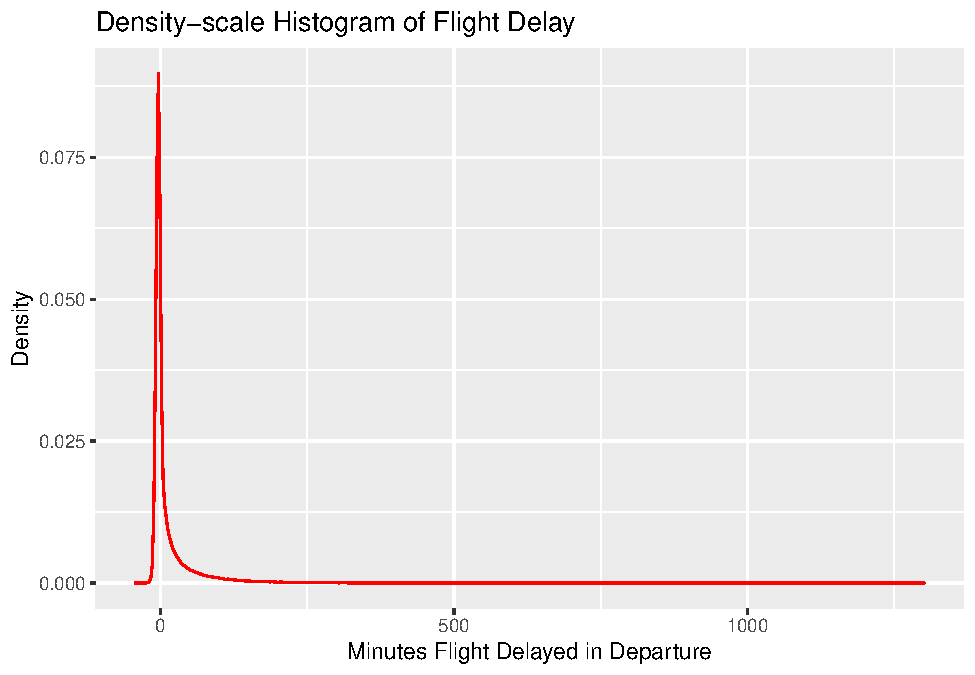
\includegraphics{DataVisua2_files/figure-latex/unnamed-chunk-6-1.pdf}

\begin{Shaded}
\begin{Highlighting}[]
\FunctionTok{ggplot}\NormalTok{(}\AttributeTok{data=}\NormalTok{demoairline1, }\AttributeTok{mapping=}\FunctionTok{aes}\NormalTok{(}\AttributeTok{x=}\NormalTok{dep\_delay)) }\SpecialCharTok{+} \FunctionTok{geom\_density}\NormalTok{(}\AttributeTok{col=}\StringTok{\textquotesingle{}red\textquotesingle{}}\NormalTok{, }\AttributeTok{na.rm=}\ConstantTok{TRUE}\NormalTok{) }\SpecialCharTok{+} \FunctionTok{xlab}\NormalTok{(}\StringTok{"Minutes Flight Delayed in Departure"}\NormalTok{) }\SpecialCharTok{+} \FunctionTok{ylab}\NormalTok{(}\StringTok{"Density"}\NormalTok{) }\SpecialCharTok{+} \FunctionTok{ggtitle}\NormalTok{(}\StringTok{"Density{-}scale Histogram of Flight Delay"}\NormalTok{)}
\end{Highlighting}
\end{Shaded}

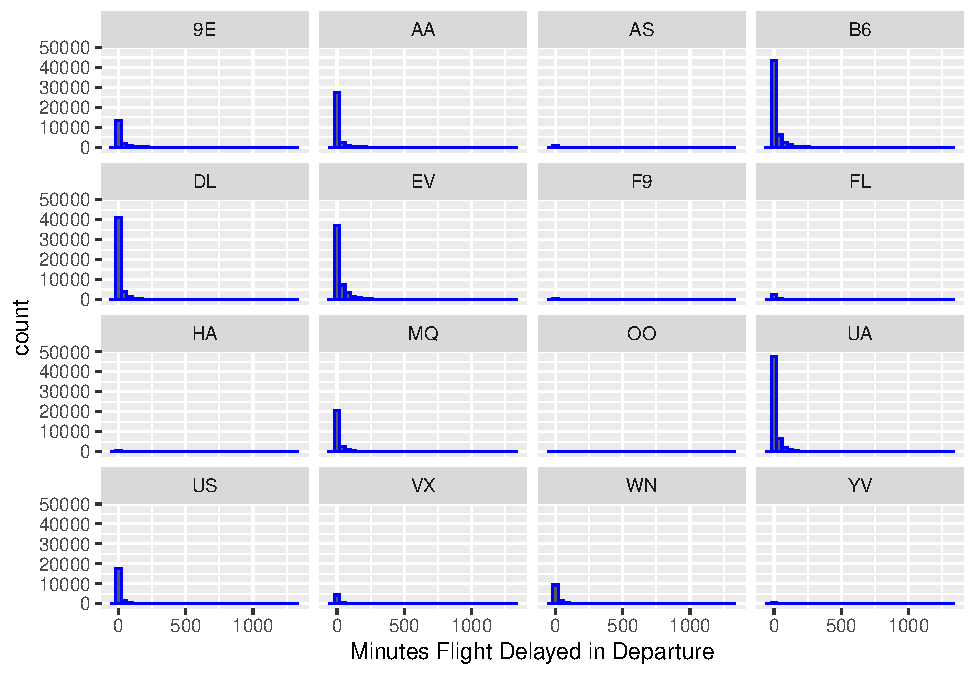
\includegraphics{DataVisua2_files/figure-latex/unnamed-chunk-7-1.pdf}

\begin{Shaded}
\begin{Highlighting}[]
\FunctionTok{ggplot}\NormalTok{(}\AttributeTok{data=}\NormalTok{demoairline1, }\AttributeTok{mapping=}\FunctionTok{aes}\NormalTok{(}\AttributeTok{x=}\NormalTok{dep\_delay)) }\SpecialCharTok{+} \FunctionTok{geom\_histogram}\NormalTok{(}\AttributeTok{col=}\StringTok{\textquotesingle{}blue\textquotesingle{}}\NormalTok{, }\AttributeTok{binwidth=}\DecValTok{40}\NormalTok{, }\AttributeTok{na.rm=}\ConstantTok{TRUE}\NormalTok{) }\SpecialCharTok{+} \FunctionTok{xlab}\NormalTok{(}\StringTok{"Minutes Flight Delayed in Departure"}\NormalTok{) }\SpecialCharTok{+} \FunctionTok{facet\_wrap}\NormalTok{(}\SpecialCharTok{\textasciitilde{}}\NormalTok{carrier)}
\end{Highlighting}
\end{Shaded}

\includegraphics{DataVisua2_files/figure-latex/unnamed-chunk-8-1.pdf}

\begin{Shaded}
\begin{Highlighting}[]
\FunctionTok{length}\NormalTok{(demoairline1}\SpecialCharTok{$}\NormalTok{dep\_delay)  }\CommentTok{\#counts the number of data points in the variable "dep\_delay"}
\end{Highlighting}
\end{Shaded}

\begin{verbatim}
## [1] 336776
\end{verbatim}

\begin{Shaded}
\begin{Highlighting}[]
\DocumentationTok{\#\# [1] 336776}
\FunctionTok{count}\NormalTok{(}\FunctionTok{is.na}\NormalTok{(demoairline1}\SpecialCharTok{$}\NormalTok{dep\_delay)) }\CommentTok{\#is.na will return each data point as TRUE if there is a N/A (missing data point)}
\end{Highlighting}
\end{Shaded}

\begin{verbatim}
##       x   freq
## 1 FALSE 328521
## 2  TRUE   8255
\end{verbatim}

\begin{Shaded}
\begin{Highlighting}[]
\DocumentationTok{\#\# n\_TRUE }
\DocumentationTok{\#\#   8255}
\CommentTok{\#or we can use the ‘filter’ function to visualize the minutes a departing flight is delayed for a certain airline, in the instance below UA (United Airlines) in addition to setting the class limits to: 0\textless{}25, 25\textless{}50, ⋯, 475\textless{}500. The earliest departure delay is {-}20 minutes, the latest is 486 minutes.}

\NormalTok{ua.breaks }\OtherTok{\textless{}{-}} \FunctionTok{seq}\NormalTok{(}\SpecialCharTok{{-}}\DecValTok{25}\NormalTok{, }\DecValTok{500}\NormalTok{, }\DecValTok{25}\NormalTok{)}
\NormalTok{ua.breaks}
\end{Highlighting}
\end{Shaded}

\begin{verbatim}
##  [1] -25   0  25  50  75 100 125 150 175 200 225 250 275 300 325 350 375 400 425
## [20] 450 475 500
\end{verbatim}

\begin{Shaded}
\begin{Highlighting}[]
\CommentTok{\#定好每个bar都是一样大小,25}
\end{Highlighting}
\end{Shaded}

\begin{Shaded}
\begin{Highlighting}[]
\FunctionTok{ggplot}\NormalTok{(}\AttributeTok{data =} \FunctionTok{filter}\NormalTok{(demoairline1, carrier }\SpecialCharTok{==} \StringTok{"UA"}\NormalTok{), }\FunctionTok{aes}\NormalTok{(}\AttributeTok{x =}\NormalTok{ dep\_delay)) }\SpecialCharTok{+} \FunctionTok{geom\_histogram}\NormalTok{(}\AttributeTok{col=}\StringTok{"red"}\NormalTok{, }\AttributeTok{fill=}\StringTok{"blue"}\NormalTok{, }\AttributeTok{breaks =}\NormalTok{ ua.breaks, }\AttributeTok{na.rm=}\ConstantTok{TRUE}\NormalTok{) }\SpecialCharTok{+} \FunctionTok{xlab}\NormalTok{(}\StringTok{"Minutes Flight Delayed in Departure"}\NormalTok{) }\SpecialCharTok{+} \FunctionTok{ylab}\NormalTok{(}\StringTok{"Count"}\NormalTok{) }\SpecialCharTok{+} \FunctionTok{ggtitle}\NormalTok{(}\StringTok{"Frequency Histogram for Departure Delay: United Airlines"}\NormalTok{)}
\end{Highlighting}
\end{Shaded}

\includegraphics{DataVisua2_files/figure-latex/unnamed-chunk-10-1.pdf}

\begin{Shaded}
\begin{Highlighting}[]
\NormalTok{delay.breaks }\OtherTok{\textless{}{-}} \FunctionTok{seq}\NormalTok{(}\SpecialCharTok{{-}}\DecValTok{100}\NormalTok{, }\DecValTok{1272}\NormalTok{, }\DecValTok{25}\NormalTok{)}


\FunctionTok{ggplot}\NormalTok{(}\AttributeTok{data=}\NormalTok{demoairline1, }\AttributeTok{mapping=}\FunctionTok{aes}\NormalTok{(}\AttributeTok{x=}\NormalTok{arr\_delay)) }\SpecialCharTok{+} \FunctionTok{geom\_histogram}\NormalTok{(}\AttributeTok{col=}\StringTok{"red"}\NormalTok{, }\AttributeTok{fill=}\StringTok{\textquotesingle{}blue\textquotesingle{}}\NormalTok{, }\AttributeTok{breaks =}\NormalTok{ delay.breaks, }\AttributeTok{na.rm=}\ConstantTok{TRUE}\NormalTok{) }\SpecialCharTok{+} \FunctionTok{xlab}\NormalTok{(}\StringTok{"Minutes Flight Delayed in Arr"}\NormalTok{) }\SpecialCharTok{+} \FunctionTok{ggtitle}\NormalTok{(}\StringTok{"Frequency Histogram of Flight arr Delay"}\NormalTok{)}
\end{Highlighting}
\end{Shaded}

\includegraphics{DataVisua2_files/figure-latex/unnamed-chunk-11-1.pdf}

\begin{Shaded}
\begin{Highlighting}[]
\NormalTok{ua.flights }\OtherTok{\textless{}{-}} \FunctionTok{subset}\NormalTok{(demoairline1, carrier }\SpecialCharTok{==} \StringTok{"UA"}\NormalTok{)}
\FunctionTok{head}\NormalTok{(ua.flights, }\DecValTok{4}\NormalTok{)}
\end{Highlighting}
\end{Shaded}

\begin{verbatim}
## # A tibble: 4 x 7
##    year month   day dep_delay carrier arr_delay distance
##   <int> <int> <int>     <dbl> <chr>       <dbl>    <dbl>
## 1  2013     1     1         2 UA             11     1400
## 2  2013     1     1         4 UA             20     1416
## 3  2013     1     1        -4 UA             12      719
## 4  2013     1     1        -2 UA              7     2475
\end{verbatim}

\begin{Shaded}
\begin{Highlighting}[]
\FunctionTok{length}\NormalTok{(demoairline1}\SpecialCharTok{$}\NormalTok{dep\_delay)}
\end{Highlighting}
\end{Shaded}

\begin{verbatim}
## [1] 336776
\end{verbatim}

\begin{Shaded}
\begin{Highlighting}[]
\FunctionTok{count}\NormalTok{(}\FunctionTok{is.na}\NormalTok{(ua.flights}\SpecialCharTok{$}\NormalTok{dep\_delay)) }
\end{Highlighting}
\end{Shaded}

\begin{verbatim}
##       x  freq
## 1 FALSE 57979
## 2  TRUE   686
\end{verbatim}

\begin{Shaded}
\begin{Highlighting}[]
\CommentTok{\#What proportion of all flights leaving the three NYC{-}area airports arrive early?}
\FunctionTok{length}\NormalTok{(demoairline1}\SpecialCharTok{$}\NormalTok{arr\_delay)}
\end{Highlighting}
\end{Shaded}

\begin{verbatim}
## [1] 336776
\end{verbatim}

\begin{Shaded}
\begin{Highlighting}[]
\FunctionTok{count}\NormalTok{(}\FunctionTok{is.na}\NormalTok{(demoairline1}\SpecialCharTok{$}\NormalTok{arr\_delay))}
\end{Highlighting}
\end{Shaded}

\begin{verbatim}
##       x   freq
## 1 FALSE 327346
## 2  TRUE   9430
\end{verbatim}

\begin{Shaded}
\begin{Highlighting}[]
\NormalTok{flight.denominator }\OtherTok{\textless{}{-}} \FunctionTok{length}\NormalTok{(demoairline1}\SpecialCharTok{$}\NormalTok{arr\_delay) }\SpecialCharTok{{-}} \FunctionTok{count}\NormalTok{(}\FunctionTok{is.na}\NormalTok{(demoairline1}\SpecialCharTok{$}\NormalTok{arr\_delay))}
\NormalTok{flight.denominator}
\end{Highlighting}
\end{Shaded}

\begin{verbatim}
##        x   freq
## 1 336776   9430
## 2 336775 327346
\end{verbatim}

\begin{Shaded}
\begin{Highlighting}[]
\FunctionTok{nrow}\NormalTok{(}\FunctionTok{subset}\NormalTok{(demoairline1,arr\_delay}\SpecialCharTok{\textless{}}\DecValTok{0}\NormalTok{))}
\end{Highlighting}
\end{Shaded}

\begin{verbatim}
## [1] 188933
\end{verbatim}

\begin{Shaded}
\begin{Highlighting}[]
\NormalTok{prop\_early }\OtherTok{\textless{}{-}}\NormalTok{ (}\FunctionTok{nrow}\NormalTok{(}\FunctionTok{subset}\NormalTok{(demoairline1,arr\_delay}\SpecialCharTok{\textless{}}\DecValTok{0}\NormalTok{)))}\SpecialCharTok{/}\NormalTok{flight.denominator}
\NormalTok{prop\_early}
\end{Highlighting}
\end{Shaded}

\begin{verbatim}
##           x       freq
## 1 0.5610049 20.0353128
## 2 0.5610066  0.5771661
\end{verbatim}

\begin{Shaded}
\begin{Highlighting}[]
\FunctionTok{ggplot}\NormalTok{(}\AttributeTok{data =} \FunctionTok{filter}\NormalTok{(demoairline1, carrier }\SpecialCharTok{==} \StringTok{"AA"}\NormalTok{), }\FunctionTok{aes}\NormalTok{(}\AttributeTok{x =}\NormalTok{ dep\_delay)) }\SpecialCharTok{+} \FunctionTok{geom\_histogram}\NormalTok{(}\AttributeTok{col=}\StringTok{"red"}\NormalTok{, }\AttributeTok{fill=}\StringTok{"blue"}\NormalTok{, }\AttributeTok{breaks =}\NormalTok{ ua.breaks, }\AttributeTok{na.rm=}\ConstantTok{TRUE}\NormalTok{) }\SpecialCharTok{+} \FunctionTok{xlab}\NormalTok{(}\StringTok{"Minutes Flight Delayed in Departure"}\NormalTok{) }\SpecialCharTok{+} \FunctionTok{ylab}\NormalTok{(}\StringTok{"Count"}\NormalTok{) }\SpecialCharTok{+} \FunctionTok{ggtitle}\NormalTok{(}\StringTok{"Frequency Histogram for Departure Delay: American Airlines"}\NormalTok{)}
\end{Highlighting}
\end{Shaded}

\includegraphics{DataVisua2_files/figure-latex/unnamed-chunk-15-1.pdf}

\begin{Shaded}
\begin{Highlighting}[]
\NormalTok{aa.flights }\OtherTok{\textless{}{-}} \FunctionTok{subset}\NormalTok{(demoairline1,carrier}\SpecialCharTok{==}\StringTok{"AA"}\NormalTok{)}
\FunctionTok{dim}\NormalTok{(aa.flights)}
\end{Highlighting}
\end{Shaded}

\begin{verbatim}
## [1] 32729     7
\end{verbatim}

\begin{Shaded}
\begin{Highlighting}[]
\FunctionTok{head}\NormalTok{(aa.flights,}\DecValTok{4}\NormalTok{)}
\end{Highlighting}
\end{Shaded}

\begin{verbatim}
## # A tibble: 4 x 7
##    year month   day dep_delay carrier arr_delay distance
##   <int> <int> <int>     <dbl> <chr>       <dbl>    <dbl>
## 1  2013     1     1         2 AA             33     1089
## 2  2013     1     1        -2 AA              8      733
## 3  2013     1     1        -1 AA             31     1389
## 4  2013     1     1        -4 AA            -12     1085
\end{verbatim}

\begin{Shaded}
\begin{Highlighting}[]
\FunctionTok{count}\NormalTok{(}\FunctionTok{is.na}\NormalTok{(aa.flights}\SpecialCharTok{$}\NormalTok{arr\_delay))}
\end{Highlighting}
\end{Shaded}

\begin{verbatim}
##       x  freq
## 1 FALSE 31947
## 2  TRUE   782
\end{verbatim}

\begin{Shaded}
\begin{Highlighting}[]
\FunctionTok{length}\NormalTok{(aa.flights}\SpecialCharTok{$}\NormalTok{arr\_delay)}
\end{Highlighting}
\end{Shaded}

\begin{verbatim}
## [1] 32729
\end{verbatim}

\begin{Shaded}
\begin{Highlighting}[]
\NormalTok{aa.flight.denominator}\OtherTok{\textless{}{-}} \FunctionTok{length}\NormalTok{(aa.flights}\SpecialCharTok{$}\NormalTok{arr\_delay)}\SpecialCharTok{{-}}\FunctionTok{count}\NormalTok{(}\FunctionTok{is.na}\NormalTok{(aa.flights}\SpecialCharTok{$}\NormalTok{arr\_delay))}
\NormalTok{aa.flight.denominator}
\end{Highlighting}
\end{Shaded}

\begin{verbatim}
##       x  freq
## 1 32729   782
## 2 32728 31947
\end{verbatim}

\begin{Shaded}
\begin{Highlighting}[]
\FunctionTok{table}\NormalTok{(demoairline1}\SpecialCharTok{$}\NormalTok{carrier)  }\CommentTok{\#creates a table counting no. flights for each carrier}
\end{Highlighting}
\end{Shaded}

\begin{verbatim}
## 
##    9E    AA    AS    B6    DL    EV    F9    FL    HA    MQ    OO    UA    US 
## 18460 32729   714 54635 48110 54173   685  3260   342 26397    32 58665 20536 
##    VX    WN    YV 
##  5162 12275   601
\end{verbatim}

\begin{Shaded}
\begin{Highlighting}[]
\CommentTok{\#frequency}
\FunctionTok{ggplot}\NormalTok{(}\AttributeTok{data=}\NormalTok{demoairline1) }\SpecialCharTok{+} \FunctionTok{geom\_bar}\NormalTok{(}\AttributeTok{mapping=}\FunctionTok{aes}\NormalTok{(}\AttributeTok{x=}\NormalTok{carrier, }\AttributeTok{fill=}\NormalTok{carrier)) }\SpecialCharTok{+} \FunctionTok{xlab}\NormalTok{(}\StringTok{"Passenger Carrier"}\NormalTok{) }\SpecialCharTok{+} \FunctionTok{ggtitle}\NormalTok{(}\StringTok{"Bar Graph of the Frequency of Departures per Carrier"}\NormalTok{)}
\end{Highlighting}
\end{Shaded}

\includegraphics{DataVisua2_files/figure-latex/unnamed-chunk-18-1.pdf}

\begin{Shaded}
\begin{Highlighting}[]
\CommentTok{\#proportion}
\FunctionTok{ggplot}\NormalTok{(}\AttributeTok{data=}\NormalTok{demoairline1) }\SpecialCharTok{+} \FunctionTok{geom\_bar}\NormalTok{(}\AttributeTok{mapping=}\FunctionTok{aes}\NormalTok{(}\AttributeTok{x=}\NormalTok{carrier ,}\AttributeTok{y=}\NormalTok{..prop.., }\AttributeTok{group=}\DecValTok{1}\NormalTok{, }\AttributeTok{fill=}\NormalTok{carrier)) }\SpecialCharTok{+} \FunctionTok{xlab}\NormalTok{(}\StringTok{"Passenger Carrier"}\NormalTok{) }\SpecialCharTok{+} \FunctionTok{ggtitle}\NormalTok{(}\StringTok{"Bar Graph of the Proportion of Departures per Carrier"}\NormalTok{)}
\end{Highlighting}
\end{Shaded}

\includegraphics{DataVisua2_files/figure-latex/unnamed-chunk-19-1.pdf}

\begin{Shaded}
\begin{Highlighting}[]
\CommentTok{\#rotation}
\FunctionTok{ggplot}\NormalTok{(}\AttributeTok{data=}\NormalTok{demoairline1) }\SpecialCharTok{+} \FunctionTok{geom\_bar}\NormalTok{(}\AttributeTok{mapping=}\FunctionTok{aes}\NormalTok{(}\AttributeTok{x=}\NormalTok{carrier ,}\AttributeTok{y=}\NormalTok{..prop.., }\AttributeTok{fill=}\NormalTok{carrier, }\AttributeTok{group=}\DecValTok{1}\NormalTok{)) }\SpecialCharTok{+} \FunctionTok{ggtitle}\NormalTok{(}\StringTok{"Bar Graph of the Proportion of Departures per Carrier"}\NormalTok{) }\SpecialCharTok{+} \FunctionTok{coord\_flip}\NormalTok{()}
\end{Highlighting}
\end{Shaded}

\includegraphics{DataVisua2_files/figure-latex/unnamed-chunk-20-1.pdf}

\begin{Shaded}
\begin{Highlighting}[]
\CommentTok{\#sorting by frequency from lowest to highest}
\FunctionTok{options}\NormalTok{(}\AttributeTok{scipen=}\DecValTok{999}\NormalTok{)}
\NormalTok{counts }\OtherTok{=} \FunctionTok{as.data.frame}\NormalTok{(}\FunctionTok{sort}\NormalTok{(}\FunctionTok{table}\NormalTok{(demoairline1}\SpecialCharTok{$}\NormalTok{carrier))) }\CommentTok{\#create a data frame from the table() command}
\NormalTok{counts}
\end{Highlighting}
\end{Shaded}

\begin{verbatim}
##    Var1  Freq
## 1    OO    32
## 2    HA   342
## 3    YV   601
## 4    F9   685
## 5    AS   714
## 6    FL  3260
## 7    VX  5162
## 8    WN 12275
## 9    9E 18460
## 10   US 20536
## 11   MQ 26397
## 12   AA 32729
## 13   DL 48110
## 14   EV 54173
## 15   B6 54635
## 16   UA 58665
\end{verbatim}

\begin{Shaded}
\begin{Highlighting}[]
\FunctionTok{ggplot}\NormalTok{(}\AttributeTok{data=}\NormalTok{counts, }\FunctionTok{aes}\NormalTok{(}\AttributeTok{x=}\NormalTok{Var1, }\AttributeTok{y=}\NormalTok{Freq, }\AttributeTok{fill=}\NormalTok{Var1)) }\SpecialCharTok{+} \FunctionTok{geom\_bar}\NormalTok{(}\AttributeTok{stat=}\StringTok{"identity"}\NormalTok{) }\SpecialCharTok{+} \FunctionTok{xlab}\NormalTok{(}\StringTok{"Airline"}\NormalTok{) }\SpecialCharTok{+} \FunctionTok{ylab}\NormalTok{(}\StringTok{"Count"}\NormalTok{) }\SpecialCharTok{+} \FunctionTok{ggtitle}\NormalTok{(}\StringTok{"Bar Graph of Counts Departures by Carrier"}\NormalTok{)}
\end{Highlighting}
\end{Shaded}

\includegraphics{DataVisua2_files/figure-latex/unnamed-chunk-22-1.pdf}

\begin{Shaded}
\begin{Highlighting}[]
\CommentTok{\#calculate the proportion first then make picture}
\NormalTok{airprop }\OtherTok{=}\NormalTok{ counts}\SpecialCharTok{$}\NormalTok{Freq}\SpecialCharTok{/}\FunctionTok{sum}\NormalTok{(counts}\SpecialCharTok{$}\NormalTok{Freq) }\CommentTok{\#converts no of flights to proportion of flights}
\NormalTok{countswithprop }\OtherTok{=} \FunctionTok{data.frame}\NormalTok{(counts, airprop) }\CommentTok{\#create a new data frame adding airprop variable to counts}
\FunctionTok{names}\NormalTok{(countswithprop)[}\FunctionTok{names}\NormalTok{(countswithprop) }\SpecialCharTok{==} \StringTok{"Var1"}\NormalTok{] }\OtherTok{\textless{}{-}} \StringTok{"Airline"} \CommentTok{\#rename the Var1 column to Airline}
\FunctionTok{head}\NormalTok{(countswithprop, }\DecValTok{4}\NormalTok{)}
\end{Highlighting}
\end{Shaded}

\begin{verbatim}
##   Airline Freq       airprop
## 1      OO   32 0.00009501865
## 2      HA  342 0.00101551179
## 3      YV  601 0.00178456897
## 4      F9  685 0.00203399292
\end{verbatim}

\begin{Shaded}
\begin{Highlighting}[]
\FunctionTok{ggplot}\NormalTok{(}\AttributeTok{data=}\NormalTok{countswithprop, }\FunctionTok{aes}\NormalTok{(}\AttributeTok{x=}\NormalTok{Airline, }\AttributeTok{y=}\NormalTok{airprop, }\AttributeTok{fill=}\NormalTok{Airline)) }\SpecialCharTok{+} \FunctionTok{geom\_bar}\NormalTok{(}\AttributeTok{stat=}\StringTok{"identity"}\NormalTok{) }\SpecialCharTok{+} \FunctionTok{xlab}\NormalTok{(}\StringTok{"Airline"}\NormalTok{) }\SpecialCharTok{+} \FunctionTok{ylab}\NormalTok{(}\StringTok{"Proportion"}\NormalTok{) }\SpecialCharTok{+} \FunctionTok{ggtitle}\NormalTok{(}\StringTok{"Bar Graph of Proportion of Departures by Carrier"}\NormalTok{)}
\end{Highlighting}
\end{Shaded}

\includegraphics{DataVisua2_files/figure-latex/unnamed-chunk-24-1.pdf}

\begin{Shaded}
\begin{Highlighting}[]
\NormalTok{demoairline2 }\OtherTok{=} \FunctionTok{select}\NormalTok{(flights, dep\_delay, arr\_delay, carrier, distance) }\CommentTok{\#select the four named variables from flights}
\FunctionTok{head}\NormalTok{(demoairline2, }\DecValTok{5}\NormalTok{)}
\end{Highlighting}
\end{Shaded}

\begin{verbatim}
## # A tibble: 5 x 4
##   dep_delay arr_delay carrier distance
##       <dbl>     <dbl> <chr>      <dbl>
## 1         2        11 UA          1400
## 2         4        20 UA          1416
## 3         2        33 AA          1089
## 4        -1       -18 B6          1576
## 5        -6       -25 DL           762
\end{verbatim}

\begin{Shaded}
\begin{Highlighting}[]
\CommentTok{\#boxplot}
\FunctionTok{ggplot}\NormalTok{(}\AttributeTok{data=}\FunctionTok{filter}\NormalTok{(demoairline2, (carrier }\SpecialCharTok{==} \StringTok{"UA"}\NormalTok{))) }\SpecialCharTok{+} \FunctionTok{geom\_boxplot}\NormalTok{(}\AttributeTok{mapping =} \FunctionTok{aes}\NormalTok{(}\AttributeTok{x =} \StringTok{"var"}\NormalTok{, }\AttributeTok{y =}\NormalTok{ dep\_delay), }\AttributeTok{fill=} \StringTok{\textquotesingle{}blue\textquotesingle{}}\NormalTok{, }\AttributeTok{na.rm=}\ConstantTok{TRUE}\NormalTok{) }\SpecialCharTok{+} \FunctionTok{xlab}\NormalTok{(}\StringTok{""}\NormalTok{) }\SpecialCharTok{+} \FunctionTok{ylab}\NormalTok{(}\StringTok{"Minutes Flight is Delayed"}\NormalTok{) }\SpecialCharTok{+} \FunctionTok{scale\_x\_discrete}\NormalTok{(}\AttributeTok{breaks=}\ConstantTok{NULL}\NormalTok{) }\SpecialCharTok{+} \FunctionTok{ggtitle}\NormalTok{(}\StringTok{"Boxplot of Departure Delay (in minutes)"}\NormalTok{)}\CommentTok{\#gives a vertical boxplot}
\end{Highlighting}
\end{Shaded}

\includegraphics{DataVisua2_files/figure-latex/unnamed-chunk-26-1.pdf}

\begin{Shaded}
\begin{Highlighting}[]
\CommentTok{\#coord\_flip}
\FunctionTok{ggplot}\NormalTok{(}\AttributeTok{data=}\FunctionTok{filter}\NormalTok{(demoairline2, (carrier }\SpecialCharTok{==} \StringTok{"UA"}\NormalTok{))) }\SpecialCharTok{+} \FunctionTok{geom\_boxplot}\NormalTok{(}\AttributeTok{mapping =} \FunctionTok{aes}\NormalTok{(}\AttributeTok{x =} \StringTok{"var"}\NormalTok{, }\AttributeTok{y =}\NormalTok{ dep\_delay), }\AttributeTok{fill=} \StringTok{\textquotesingle{}blue\textquotesingle{}}\NormalTok{, }\AttributeTok{na.rm=}\ConstantTok{TRUE}\NormalTok{) }\SpecialCharTok{+} \FunctionTok{xlab}\NormalTok{(}\StringTok{""}\NormalTok{) }\SpecialCharTok{+} \FunctionTok{ylab}\NormalTok{(}\StringTok{"Minutes Flight is Delayed"}\NormalTok{) }\SpecialCharTok{+} \FunctionTok{scale\_x\_discrete}\NormalTok{(}\AttributeTok{breaks=}\ConstantTok{NULL}\NormalTok{) }\SpecialCharTok{+} \FunctionTok{ggtitle}\NormalTok{(}\StringTok{"Boxplot of Departure Delay (in minutes)"}\NormalTok{) }\SpecialCharTok{+} \FunctionTok{coord\_flip}\NormalTok{() }\CommentTok{\#provides a horizontal bp}
\end{Highlighting}
\end{Shaded}

\includegraphics{DataVisua2_files/figure-latex/unnamed-chunk-27-1.pdf}

\begin{Shaded}
\begin{Highlighting}[]
\CommentTok{\#2 in 1}
\FunctionTok{ggplot}\NormalTok{(}\AttributeTok{data=}\FunctionTok{filter}\NormalTok{(demoairline2, (carrier }\SpecialCharTok{==} \StringTok{"UA"} \SpecialCharTok{|}\NormalTok{ carrier}\SpecialCharTok{==}\StringTok{"AA"}\NormalTok{)), }\FunctionTok{aes}\NormalTok{(}\AttributeTok{x =}\NormalTok{ carrier, }\AttributeTok{y=}\NormalTok{arr\_delay)) }\SpecialCharTok{+} \FunctionTok{geom\_boxplot}\NormalTok{(}\AttributeTok{fill=}\StringTok{\textquotesingle{}blue\textquotesingle{}}\NormalTok{, }\AttributeTok{na.rm=}\ConstantTok{TRUE}\NormalTok{) }\SpecialCharTok{+} \FunctionTok{ggtitle}\NormalTok{(}\StringTok{"Boxplots of Departure Delays (minutes) for United Airlines and American Airlines"}\NormalTok{) }\SpecialCharTok{+} \FunctionTok{coord\_flip}\NormalTok{()}
\end{Highlighting}
\end{Shaded}

\includegraphics{DataVisua2_files/figure-latex/unnamed-chunk-28-1.pdf}

\begin{Shaded}
\begin{Highlighting}[]
\CommentTok{\#3 in 1}
\FunctionTok{ggplot}\NormalTok{(}\AttributeTok{data=}\FunctionTok{filter}\NormalTok{(demoairline2, (carrier }\SpecialCharTok{==} \StringTok{"UA"} \SpecialCharTok{|}\NormalTok{ carrier}\SpecialCharTok{==}\StringTok{"AA"} \SpecialCharTok{|}\NormalTok{ carrier }\SpecialCharTok{==} \StringTok{"B6"}\NormalTok{)), }\FunctionTok{aes}\NormalTok{(}\AttributeTok{x =}\NormalTok{ carrier, }\AttributeTok{y=}\NormalTok{arr\_delay)) }\SpecialCharTok{+} \FunctionTok{geom\_boxplot}\NormalTok{(}\AttributeTok{fill=}\StringTok{\textquotesingle{}red\textquotesingle{}}\NormalTok{, }\AttributeTok{na.rm=}\ConstantTok{TRUE}\NormalTok{) }\SpecialCharTok{+} \FunctionTok{ylab}\NormalTok{(}\StringTok{"Minutes Flight is Late in Arriving"}\NormalTok{) }\SpecialCharTok{+} \FunctionTok{ggtitle}\NormalTok{(}\StringTok{"Boxplots of Departure Arrival (minutes) for United, Jet Blue, and American Airlines from NYC Airports"}\NormalTok{)  }\SpecialCharTok{+} \FunctionTok{coord\_flip}\NormalTok{()}
\end{Highlighting}
\end{Shaded}

\includegraphics{DataVisua2_files/figure-latex/unnamed-chunk-29-1.pdf}

\begin{Shaded}
\begin{Highlighting}[]
\CommentTok{\#all in one}
\FunctionTok{ggplot}\NormalTok{(}\AttributeTok{data=}\NormalTok{demoairline2, }\FunctionTok{aes}\NormalTok{(}\AttributeTok{x=}\NormalTok{carrier, }\AttributeTok{y=}\NormalTok{dep\_delay, }\AttributeTok{color =}\NormalTok{ carrier)) }\SpecialCharTok{+} \FunctionTok{geom\_boxplot}\NormalTok{(}\AttributeTok{na.rm=}\ConstantTok{TRUE}\NormalTok{) }\SpecialCharTok{+} \FunctionTok{ylab}\NormalTok{(}\StringTok{"Minutes Flight is Delayed"}\NormalTok{)}
\end{Highlighting}
\end{Shaded}

\includegraphics{DataVisua2_files/figure-latex/unnamed-chunk-30-1.pdf}

\begin{Shaded}
\begin{Highlighting}[]
\CommentTok{\#geom\_violin}

\FunctionTok{ggplot}\NormalTok{(}\AttributeTok{data =} \FunctionTok{filter}\NormalTok{(demoairline2, carrier}\SpecialCharTok{==}\StringTok{"UA"}\NormalTok{), }\FunctionTok{aes}\NormalTok{(}\AttributeTok{x =}\NormalTok{ carrier, }\AttributeTok{y =}\NormalTok{ dep\_delay)) }\SpecialCharTok{+} \FunctionTok{geom\_violin}\NormalTok{(}\AttributeTok{col=}\StringTok{"blue"}\NormalTok{, }\AttributeTok{fill=}\StringTok{"red"}\NormalTok{, }\AttributeTok{na.rm=}\ConstantTok{TRUE}\NormalTok{) }\SpecialCharTok{+} \FunctionTok{xlab}\NormalTok{(}\StringTok{"United Airlines"}\NormalTok{) }\SpecialCharTok{+} \FunctionTok{ylab}\NormalTok{(}\StringTok{"Minutes a Departing Flight is Delayed"}\NormalTok{) }\SpecialCharTok{+} \FunctionTok{ggtitle}\NormalTok{(}\StringTok{"Violin Plot of United Airline Departure Delays: 3{-}NYC Airports"}\NormalTok{)}
\end{Highlighting}
\end{Shaded}

\includegraphics{DataVisua2_files/figure-latex/unnamed-chunk-31-1.pdf}

\begin{Shaded}
\begin{Highlighting}[]
\CommentTok{\#boxviolin}
\FunctionTok{ggplot}\NormalTok{(}\AttributeTok{data =} \FunctionTok{filter}\NormalTok{(demoairline2, carrier}\SpecialCharTok{==}\StringTok{"UA"}\NormalTok{), }\FunctionTok{aes}\NormalTok{(}\AttributeTok{x =}\NormalTok{ carrier, }\AttributeTok{y =}\NormalTok{ dep\_delay)) }\SpecialCharTok{+} \FunctionTok{geom\_violin}\NormalTok{(}\AttributeTok{col=}\StringTok{"blue"}\NormalTok{, }\AttributeTok{fill=}\StringTok{"red"}\NormalTok{, }\AttributeTok{na.rm=}\ConstantTok{TRUE}\NormalTok{) }\SpecialCharTok{+} \FunctionTok{geom\_boxplot}\NormalTok{(}\AttributeTok{width=}\FloatTok{0.1}\NormalTok{, }\AttributeTok{na.rm=}\ConstantTok{TRUE}\NormalTok{) }\SpecialCharTok{+} \FunctionTok{xlab}\NormalTok{(}\StringTok{"United Airlines"}\NormalTok{) }\SpecialCharTok{+} \FunctionTok{ylab}\NormalTok{(}\StringTok{"Minutes a Departing Flight is Delayed"}\NormalTok{) }\SpecialCharTok{+} \FunctionTok{ggtitle}\NormalTok{(}\StringTok{"Violin Plot of United Airline Departure Delays: 3{-}NYC Airports"}\NormalTok{) }\SpecialCharTok{+} \FunctionTok{coord\_flip}\NormalTok{()}
\end{Highlighting}
\end{Shaded}

\includegraphics{DataVisua2_files/figure-latex/unnamed-chunk-32-1.pdf}

\begin{Shaded}
\begin{Highlighting}[]
\NormalTok{flightstoLAX }\OtherTok{=} \FunctionTok{filter}\NormalTok{(flights, (dest}\SpecialCharTok{==}\StringTok{"LAX"}\NormalTok{)) }\CommentTok{\#filter out all destinations that are LAX}
\FunctionTok{head}\NormalTok{(flightstoLAX, }\DecValTok{4}\NormalTok{) }\CommentTok{\#a pieak at the data...}
\end{Highlighting}
\end{Shaded}

\begin{verbatim}
## # A tibble: 4 x 19
##    year month   day dep_time sched_dep~1 dep_d~2 arr_t~3 sched~4 arr_d~5 carrier
##   <int> <int> <int>    <int>       <int>   <dbl>   <int>   <int>   <dbl> <chr>  
## 1  2013     1     1      558         600      -2     924     917       7 UA     
## 2  2013     1     1      628         630      -2    1016     947      29 UA     
## 3  2013     1     1      658         700      -2    1027    1025       2 VX     
## 4  2013     1     1      702         700       2    1058    1014      44 B6     
## # ... with 9 more variables: flight <int>, tailnum <chr>, origin <chr>,
## #   dest <chr>, air_time <dbl>, distance <dbl>, hour <dbl>, minute <dbl>,
## #   time_hour <dttm>, and abbreviated variable names 1: sched_dep_time,
## #   2: dep_delay, 3: arr_time, 4: sched_arr_time, 5: arr_delay
\end{verbatim}

\begin{Shaded}
\begin{Highlighting}[]
\NormalTok{whofliestoLAX }\OtherTok{=} \FunctionTok{as.data.frame}\NormalTok{(}\FunctionTok{sort}\NormalTok{(}\FunctionTok{table}\NormalTok{(flightstoLAX}\SpecialCharTok{$}\NormalTok{carrier)))}
\NormalTok{whofliestoLAX}
\end{Highlighting}
\end{Shaded}

\begin{verbatim}
##   Var1 Freq
## 1   B6 1688
## 2   DL 2501
## 3   VX 2580
## 4   AA 3582
## 5   UA 5823
\end{verbatim}

\begin{Shaded}
\begin{Highlighting}[]
\NormalTok{sam\_flights }\OtherTok{=} \FunctionTok{sample}\NormalTok{(flights, }\DecValTok{1000}\NormalTok{, }\AttributeTok{replace=}\ConstantTok{FALSE}\NormalTok{)  }\CommentTok{\#select 1000 cases from flights without replacement}
\FunctionTok{head}\NormalTok{(sam\_flights, }\DecValTok{4}\NormalTok{) }
\end{Highlighting}
\end{Shaded}

\begin{verbatim}
## # A tibble: 4 x 20
##    year month   day dep_time sched_dep~1 dep_d~2 arr_t~3 sched~4 arr_d~5 carrier
##   <int> <int> <int>    <int>       <int>   <dbl>   <int>   <int>   <dbl> <chr>  
## 1  2013     4    26     1200        1155       5    1456    1441      15 B6     
## 2  2013     9    22      610         615      -5     748     813     -25 US     
## 3  2013     6    10     1856        1729      87    2226    2059      87 UA     
## 4  2013    11    19     1222        1215       7    1547    1550      -3 UA     
## # ... with 10 more variables: flight <int>, tailnum <chr>, origin <chr>,
## #   dest <chr>, air_time <dbl>, distance <dbl>, hour <dbl>, minute <dbl>,
## #   time_hour <dttm>, orig.id <chr>, and abbreviated variable names
## #   1: sched_dep_time, 2: dep_delay, 3: arr_time, 4: sched_arr_time,
## #   5: arr_delay
\end{verbatim}

\begin{Shaded}
\begin{Highlighting}[]
\NormalTok{nsize }\OtherTok{=} \FunctionTok{length}\NormalTok{(sam\_flights}\SpecialCharTok{$}\NormalTok{dep\_delay) }\SpecialCharTok{{-}} \FunctionTok{count}\NormalTok{(}\FunctionTok{is.na}\NormalTok{(sam\_flights}\SpecialCharTok{$}\NormalTok{dep\_delay)) }\CommentTok{\#subtracts missing values to determine n}
\NormalTok{nsize}
\end{Highlighting}
\end{Shaded}

\begin{verbatim}
##      x freq
## 1 1000   25
## 2  999  975
\end{verbatim}

\begin{Shaded}
\begin{Highlighting}[]
\FunctionTok{ggplot}\NormalTok{(sam\_flights, }\FunctionTok{aes}\NormalTok{(}\AttributeTok{x =}\NormalTok{ dep\_delay)) }\SpecialCharTok{+} \FunctionTok{geom\_histogram}\NormalTok{(}\AttributeTok{col=}\StringTok{\textquotesingle{}red\textquotesingle{}}\NormalTok{, }\AttributeTok{fill=}\StringTok{\textquotesingle{}blue\textquotesingle{}}\NormalTok{, }\AttributeTok{binwidth=}\DecValTok{20}\NormalTok{, }\AttributeTok{na.rm=}\ConstantTok{TRUE}\NormalTok{) }\SpecialCharTok{+} \FunctionTok{xlab}\NormalTok{(}\StringTok{"Minutes Flight is Delayed"}\NormalTok{)}\SpecialCharTok{+} \FunctionTok{ggtitle}\NormalTok{(}\StringTok{"Histogram of Flight Delays for Sample of 971 flights"}\NormalTok{) }\SpecialCharTok{+} \FunctionTok{geom\_vline}\NormalTok{(}\AttributeTok{xintercept =} \DecValTok{0}\NormalTok{, }\AttributeTok{col=}\StringTok{"orange"}\NormalTok{)}
\end{Highlighting}
\end{Shaded}

\includegraphics{DataVisua2_files/figure-latex/unnamed-chunk-37-1.pdf}

\begin{Shaded}
\begin{Highlighting}[]
\FunctionTok{ggplot}\NormalTok{(sam\_flights, }\FunctionTok{aes}\NormalTok{(}\AttributeTok{x =}\NormalTok{ dep\_delay, }\AttributeTok{y =}\NormalTok{..density.., }\AttributeTok{group=}\FunctionTok{as.factor}\NormalTok{(month))) }\SpecialCharTok{+} \FunctionTok{geom\_freqpoly}\NormalTok{(}\FunctionTok{aes}\NormalTok{(}\AttributeTok{color=}\FunctionTok{as.factor}\NormalTok{(month)), }\AttributeTok{binwidth=}\DecValTok{20}\NormalTok{,}\AttributeTok{na.rm=}\ConstantTok{TRUE}\NormalTok{) }
\end{Highlighting}
\end{Shaded}

\includegraphics{DataVisua2_files/figure-latex/unnamed-chunk-38-1.pdf}

\begin{Shaded}
\begin{Highlighting}[]
\NormalTok{assessedvalue}\OtherTok{=} \FunctionTok{c}\NormalTok{(}\FloatTok{342.0}\NormalTok{, }\FloatTok{166.5}\NormalTok{, }\FloatTok{406.0}\NormalTok{, }\FloatTok{303.5}\NormalTok{, }\FloatTok{704.5}\NormalTok{, }\FloatTok{540.0}\NormalTok{, }\DecValTok{373}\NormalTok{, }\FloatTok{449.5}\NormalTok{, }\FloatTok{398.5}\NormalTok{, }\FloatTok{394.5}\NormalTok{, }\DecValTok{219}\NormalTok{, }\FloatTok{220.0}\NormalTok{, }\FloatTok{398.5}\NormalTok{, }\FloatTok{480.5}\NormalTok{, }\FloatTok{364.0}\NormalTok{)}
\NormalTok{propassess }\OtherTok{=} \FunctionTok{data.frame}\NormalTok{(assessedvalue) }\CommentTok{\#create a data frame to prepare data to be visualzed wtih ggplot}
\FunctionTok{head}\NormalTok{(propassess, }\DecValTok{3}\NormalTok{)}
\end{Highlighting}
\end{Shaded}

\begin{verbatim}
##   assessedvalue
## 1         342.0
## 2         166.5
## 3         406.0
\end{verbatim}

\begin{Shaded}
\begin{Highlighting}[]
\FunctionTok{densityplot}\NormalTok{(propassess}\SpecialCharTok{$}\NormalTok{assessedvalue, }\AttributeTok{xlab=}\StringTok{"Property Assessment in $1000s"}\NormalTok{, }\AttributeTok{main=}\StringTok{"Density Plot of Residential Property Assessments"}\NormalTok{)}
\end{Highlighting}
\end{Shaded}

\includegraphics{DataVisua2_files/figure-latex/unnamed-chunk-40-1.pdf}

\begin{Shaded}
\begin{Highlighting}[]
\NormalTok{ct}\OtherTok{=} \FunctionTok{c}\NormalTok{(}\DecValTok{0}\NormalTok{,  }\DecValTok{0}\NormalTok{,  }\DecValTok{5}\NormalTok{,  }\DecValTok{6}\NormalTok{, }\DecValTok{10}\NormalTok{, }\DecValTok{10}\NormalTok{, }\DecValTok{15}\NormalTok{, }\DecValTok{15}\NormalTok{, }\DecValTok{15}\NormalTok{, }\DecValTok{20}\NormalTok{, }\DecValTok{20}\NormalTok{, }\DecValTok{25}\NormalTok{, }\DecValTok{30}\NormalTok{, }\DecValTok{40}\NormalTok{, }\DecValTok{45}\NormalTok{, }\DecValTok{60}\NormalTok{, }\DecValTok{60}\NormalTok{, }\DecValTok{60}\NormalTok{, }\DecValTok{60}\NormalTok{) }\CommentTok{\# combined these data into a data vector called ct}
\NormalTok{ct }\OtherTok{=} \FunctionTok{sort}\NormalTok{(ct)  }\CommentTok{\# arranges the data from smallest to largest}
\NormalTok{ct}\CommentTok{\# see the data in ascending value}
\end{Highlighting}
\end{Shaded}

\begin{verbatim}
##  [1]  0  0  5  6 10 10 15 15 15 20 20 25 30 40 45 60 60 60 60
\end{verbatim}

\begin{Shaded}
\begin{Highlighting}[]
\FunctionTok{mean}\NormalTok{(ct)}
\end{Highlighting}
\end{Shaded}

\begin{verbatim}
## [1] 26.10526
\end{verbatim}

\begin{Shaded}
\begin{Highlighting}[]
\FunctionTok{median}\NormalTok{(ct)}
\end{Highlighting}
\end{Shaded}

\begin{verbatim}
## [1] 20
\end{verbatim}

\end{document}
